\chapter{示例章节}
示例文字:跟着我左手右手一个慢动作
\section{示例小节}
示例文字:右手左右慢动作重复播
\subsection{示例条}
示例文字:这首歌\\ 给你快乐\\ 你有没有爱上我\footnote{tfboys的歌,你还好吗?},哈哈

\begin{enumerate}[leftmargin=24pt]
	\item 昨天所有的荣耀
	\item 已变成遥远的回忆
	\item 辛辛苦苦,已度过半生
	\item 今夜重又走进风雨
\end{enumerate}

\begin{figure}[H]
	\centering
	\begin{subfigure}[b]{0.3\textwidth}
		\centering
		
\includegraphics[width=.15\textheight]{images/make_a_big_news.jpg}
		\caption{弄个大新闻}
	\end{subfigure}
	\begin{subfigure}[b]{0.3\textwidth}
		\centering
		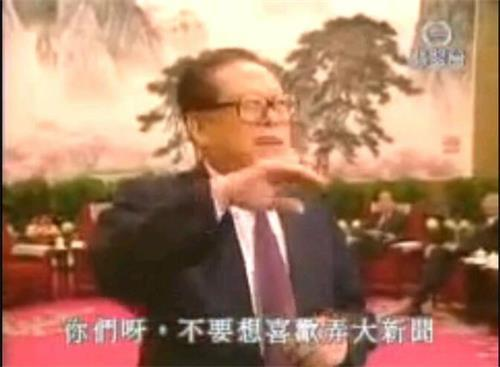
\includegraphics[width=.15\textheight]{images/you_like_big_news.jpg}
		\caption{不要想喜欢弄大新闻}
	\end{subfigure}
	\caption{我为长者续一秒}
\end{figure}

{\wuhao 五号字体}

{\CJKfamily{Heiti} 然后搞点黑体}

举个文献的栗子\footnote{感谢提供:https://github.com/Haixing-Hu/GBT7714-2005-BibTeX-Style}:诸葛亮写了本书叫《论六出祁山的必要性与可行性》\textsuperscript{\cite{诸葛亮:Book}},然后发了篇文章\cite{诸葛亮:Article},然后刘备就长坂坡摔小孩了\textsuperscript{\cite{刘备:摔小孩}}\footnote{例子原型:http://lyanry.is-programmer.com/posts/195.html}

\subsection{又来一节}
你的头发还好好吗?
